\documentclass{article}

\usepackage{amsmath}
\usepackage{graphicx}
\usepackage{float}

\title{Sul diagramma di Mollier e le isobariche}
\author{Amro Awad Saad Moustafa Soliman}

\begin{document}
\maketitle
Si vuole dimostrare che nel diagramma di Mollier, a parità di entalpia, le isobariche assumono valori di pressione decrescenti nella direzione di crescita della entropia, e che, a parità di entropia, le isobariche assumono valori di pressione crescenti nella direzione di crescita dell'entalpia.

Essendo le tre varibili analizzate sono l'entalpia $h$, l'entropia $s$ e la pressione $p$, si può ricorrere alla formulazione differenziale di $h=h(s,p)$:
\begin{equation}
  dh=Tds+vdp
\end{equation}
Per primo, si consideri il caso isoentalpico. Dato che l'entalpia è costante, e cioè $dh=0$, la $(1)$ diventa:
\begin{equation}
  Tds=-vdp
\end{equation}
dove la temperatura $T$ e il volume $v$ sono grandezze positive per definizione.
Dunque una variazione positiva dell'entropia, a parità di entalpia, implica una diminuzione della pressione.

Ora, si consideri il caso isoentropico. Essendo l'entropia costante, e cioè $ds=0$, la $(1)$ assume la forma:
\begin{equation}
  dh=vdp
\end{equation}
\begin{figure}[H]
  \centering
  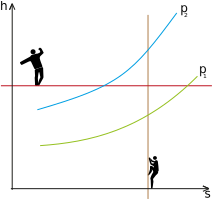
\includegraphics[scale=0.85]{Grafico_di_Mollier.png}
\end{figure}
Il che significa che un aumento dell'entalpia, a parità di entropia, corrisponde a un aumento della pressione.

In termini intuitivi, la dimostrazione può essere visualizzata introducendo due personaggi: il \textit{funambolo isoentalpico} e lo \textit{scalatore isoentropico}.
Il funambolo isoentalpico, essendo vincolato a seguire una traiettoria orizzontale, procedendo verso destra del diagramma di Mollier e analizzando la $(2)$ nota che incontra isobariche con pressioni man mano decrescenti. Invece, lo scalatore isoentropico, essendo vincolato alla traiettoria verticale, man mano che procede verso l'alto nota che secondo la $(3)$ incontra isobariche con pressioni crescenti.
\end{document}
